\chapter{BJT Common Emitter Characteristics}
	\section{Aim}
		\begin{itemize}
			\tightlist
			\item Explain structure of Bipolar Junction Transistor
			\item Explain Operation of Bipolar Junction Transistor
			\item Explain Common Emitter characteristics of a BJT
		\end{itemize}
	
	\section{Apparatus}
		\begin{itemize}
			\tightlist
			\item A Bipolar Junction Transistor
			\item Voltmeter
			\item Ammeter
			\item Rheostat
			\item Battery
		\end{itemize}
	
	\section{Theory}
		\subsection{Structure of Bipolar Junction Transistor}
			A bipolar junction transistor, BJT, is a single piece of silicon with two back-to-back P-N junctions.BJTs can be made either as PNP or as NPN.
			\begin{figure}[h]
				\centering
				
\includegraphics[width=0.5\linewidth]{img/exp9/1}
				\caption{Structures, layers and circuit symbol of NPN transistor}
				\label{fig:bjt_npn}
			\end{figure}
			
			They have three regions and three terminals, emitter, base, and collector represented by E, B, and C respectively. The direction of the arrow indicates the direction of the current in the emitter when the transistor is conducting normally. An easy way to remember this is NPN stands for "Not Pointing iN".
			\begin{figure}[h]
				\centering
				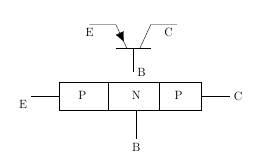
\includegraphics[width=0.5\linewidth]{img/exp9/2}
				\caption{Structures, layers and circuit symbol of PNP transistor}
				\label{fig:bjt_pnp}
			\end{figure}
		
			\textbf{Emitter (E)}:It is the region to the left end which supply free charge carriers i.e., electrons in n-p-n or holes in p-n-p transistors.These majority carriers are injected to the middle region i.e. electrons in the p region of n-p-n or holes in the n region of p-n-p transistor. Emitter is a heavily doped region to supply a large number of majority carriers into the base.
			
			\textbf{Base (B)}:It is the middle region where either two p-type layers or two n-type layers are sandwiched. The majority carriers from the emitter region are injected into this rgion.This region is thin and very lightly doped.
			
			\textbf{Collector (C)}:It is the region to right end where charge carriers are collected.The area of this region is largest compared to emitter and base region . The doping level of this region is intermediate between heavily doped emitter region and lightly doped base region.
			
		\subsection{Operation of Bipolar Junction Transistor}
			\begin{figure}[h]
				\centering
				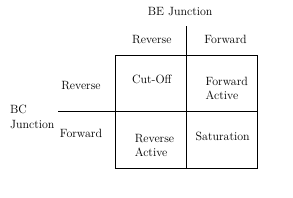
\includegraphics[width=0.7\linewidth]{img/exp9/3}
				\caption{Four Operating Conditions}
				\label{fig:bjt_op_conditions}
			\end{figure}
			\textbf{Cutoff Region}: Base-emitter junction is reverse biased. No current flow.
			
			\textbf{Saturation Region}: Base-emitter junction is forward biased and Collector-base junction is forward biased.
			
			\textbf{Active Region}: Base-emitter is junction forward biased and Collector-base junction is reverse biased.
			
			\textbf{Breakdown Region}: \(I_C\) and \(V_{CE}\) exceed specifications and can cause damage to the transistor.
			
		\subsection{Cut-Off Region}
			In Cut-Off region both junctions are reverse biased, Base-emitter junction is reverse biased (\(V_{BE}<0\))and also Collector-Base junction is reverse biased(\(V_{CB}>0\)).With reverse biasing, all currents are zero.There are some leakage currents associated with reverse biased junctions,but these currents are small and therefore can be neglected.
		
		\subsection{Forward Active Region}
			In Forward Active region Base-emitter junction is forward biased(\(V_{BE}>0\)) and Collector-Base junction is reverse biased(\(V_{CB}>0\)). In this case, the forward bias of the BE junction will cause the injection of both holes and electrons across the junction. The holes are of little consequence because the doping levels are adjusted to minimize the hole current. The electrons are the carriers of interest. The electrons are injected into the base region where they are called the minority carrier even though they greatly outnumber the holes.
			Application:Amplifier in analog circuits						
			$$I_C= -\alpha_F \times I_E + I_{CO}$$
			where,
			\(\alpha_F\) is the forward current transfer ratio
			\(I_{CO}\) is Collector reverse saturation current
		
		\subsection{Saturation Region}
			In Saturation region both junctions are Forward biased,Base-emitter junction is forward biased(\(V_{BE}>0\)) and also Collector-Base junction is forward biased(\(V_{CB}<0\)). Maximum currents flows through the transistor with only a small voltage drop across the collector junction.The transistor also does not respond to any change in emitter current or base-emitter voltage.
		
		\subsection{Reverse Active Region}
			In Reverse Active region Base-emitter junction is reverse biased(\(V_{BE}<0\)) and Collector-Base junction is forward biased(\(V_{CB}<0\)).The operation is just the same as the forward active region, except all voltage sources, and hence collector and emitter currents, are the reverse of the forward bias case. The current gain in this mode is smaller than that of forward active mode for which this mode in general unsuitable for amplification.
			Application:In digital circuits and analog switching circuits.						
			$$I_E = -\alpha_R* I_C + I_{EO}$$ where,
			\(\alpha_R\) is the reverse current transfer ratio\newline \(I_{EO}\) is the Emitter reverse saturation current
			
			This configuration is rarely used because most transistors are doped selectively to give forward current transfer ratios very near unity, which automatically causes the reverse current transfer ratio to be very low.
		
		\subsection{BJT - Common Emitter Circuit}
			The DC behavior of the BJT can be described by the Ebers-Moll Model. The equations for the model are:
			$$I_F= I_{ES} \times ( exp^ \frac{V_{BE}}{V_T} -1)$$
			$$I_R= I_{CS} \times(exp^ \frac{V_{CB}}{V_T} -1)$$ where,
			\(I _{ES}\) is base-emitter saturation currents,\\
			\(I_{CS}\) is base-collector saturation currents
			$$V_T = \frac{k \times T}{q}$$
			where,
			k is the Boltzmann’s constant ( k = 1.381 e-23 V.C/ K ),\\
			T is the absolute temperature in degrees Kelvin, and\\
			q is the charge of an electron (q = 1.602 e-19 C).			
			$$\beta_F = \frac{\alpha_F}{1 - \alpha_F}$$ $$\beta_R= \frac{\alpha_R}{1 - \alpha_R}$$
			where,\\
			\(\beta_F\) is large signal forward current gain of common-emitter configuration,\\
			\(\beta_R\) is the large signal reverse current gain of the common-emitter configuration
			$$ \alpha_F=\frac{\beta_F}{1 + \beta_F}$$
			$$\alpha_R=\frac{\beta_R}{1 + \beta_R}$$
			where,\\
			\(\alpha_R\) is large signal reverse current gain of a common-base configuration,\\
			\(\alpha_F\) is large signal forward current gain of the common-base configuration.
			$$I_C = \alpha_F \times I_F - I_R$$
			$$ I_E = -I_F + \alpha_R * I_R$$
			$$ I_B = (1 - \alpha_F) \times I_F + (1 - \alpha_R) \times I_R$$
			The forward and reverse current gains are related by the expression
			$$ \alpha_R \times I_{CS}=\alpha_F \times I_{ ES} =I_S$$
			where,\\
			\(I_S\) is the BJT transport saturation current.\\
			The parameters \(\alpha_R\) and \(\alpha_F\) are influenced by impurity concentrations and junction depths.\\
			The saturation current, \(I_S\) , can be expressed as
			$$ I_S = J_S \times A$$
			where,\\
			A is the area of the emitter and\\
			\(J_S\) is the transport saturation current density
		
		\subsection{Input Characteristics}
			The most important characteristic of the BJT is the plot of the base current, \(I_B\), versus the base-emitter voltage,\(V_{BE}\), for various values of the collector-emitter voltage,\(V_{CE}\)		
			
			$$I_B=\phi (V_{BE},V_{CE}) \qquad for\quad constant \quad V_{CE}$$
			\begin{figure}[h]
				\centering
				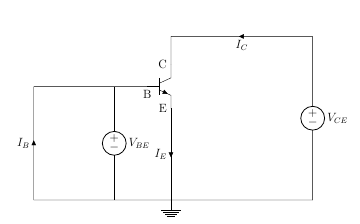
\includegraphics[width=0.7\linewidth]{img/exp9/4}
				\caption{Input Characteristics Circuit}
				\label{fig:bjt_inputCircuit}
			\end{figure}
		
		\subsection{Output Characteristics}
			The most important characteristic of the BJT is the plot of the collector current, $I_C$, versus the collector-emitter voltage,$V_{CE}$, for various values of the base current, $I_B$ as shown on the circuit on the right.						
			$$I_C =\phi(V_{CE} , I_B) \qquad for\quad constant \quad I_B $$
			\begin{figure}[h]
				\centering
				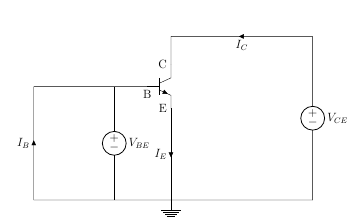
\includegraphics[width=0.7\linewidth]{img/exp9/5}
				\caption{Output Characteristics Circuit}
				\label{fig:bjt_outputCircuit}
			\end{figure}
		
	\section{Procedure}
		\subsection{BJT Common Emitter - Input Characteristics}
			\begin{enumerate}
				\tightlist
				\item Initially set rheostat $R_{h1} = 1\Omega$ and rheostat $R_{h2} = 1\Omega$
				\item Set the Collector-Emitter Voltage($V_{CE}$) to 1V by adjusting the rheostat $R_{h2}$
				\item Base Emitter Voltage($V_{BE}$) is varied by adjusting the rheostat $R_{h1}$.
				\begin{figure}[h]
					\centering
					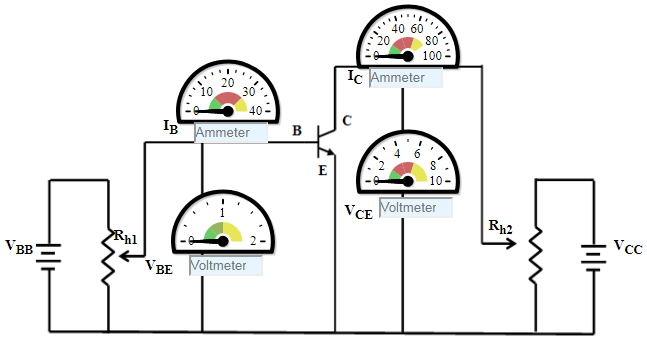
\includegraphics[width=0.7\linewidth]{img/exp9/6}
					\caption{Simulation for BJT Common Emitter - Input Characteristics}
					\label{fig:bjt_procedure_input}
				\end{figure}
				\item Note the reading of Base current($I_B$)in micro Ampere.
				\item Click on 'Plot' to plot the I-V characteristics of Common - Emitter configuration. A graph is drawn with VBE along X-axis and $I_B$ along Y-axis.
				\item Click on 'Clear' button to take another sets of readings
				\item Now set the Collector-Emitter Voltage($V_{CE}$) to 2V, 3V, 4V
			\end{enumerate}
		
		\subsection{BJT Common Emitter - Output Characteristics}
			\begin{enumerate}
				\tightlist
				\item Initially set rheostat $R_{h1} = 1\Omega$ and rheostat $R_{h2} = 1\Omega$
				\item Set the Base current($I_B$) $15\mu A$ by adjusting the rheostat $R_{h1}$
				\begin{figure}[h]
					\centering
					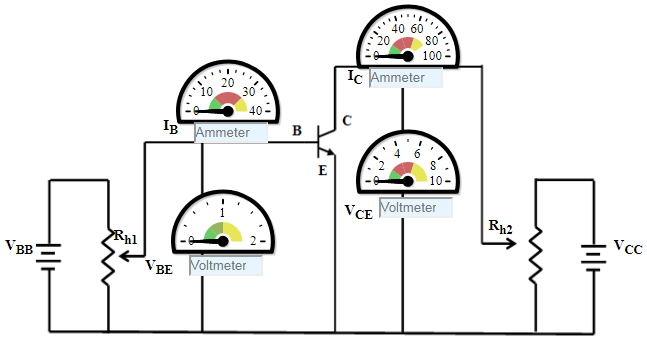
\includegraphics[width=0.7\linewidth]{img/exp9/7}
					\caption{Simulation for BJT Common Emitter - Output Characteristics}
					\label{fig:bjt_procedure_output}
				\end{figure}
				\item Vary the Collector-Emitter Voltage($V_{CE}$)is varied by adjusting the rheostat $R_{h2}$.
				\item Note the reading of Collector current($I_C$).
				\item Click on 'Plot' to plot the I-V characteristics of Common - Emitter configuration. A graph is drawn with $V_{CE}$ along X-axis and $I_C$ along Y-axis.
				\item Click on 'Clear' button to take another sets of readings
				\item Now set the Base Current($I_B$) to $20\mu A$
			\end{enumerate}
	
	\section{Observations}
		\subsection{BJT Common Emmiter - Input Characteristics}
			\begin{figure}[h]
				\begin{longtable}[]{@{}lll@{}}
					\toprule
					Sr No. & Base-Emitter Voltage ($V$) & Base Current ($\mu A$)\tabularnewline
					\midrule
					\endhead
					1 & 0.06000 & 2.179\tabularnewline
					2 & 0.2400 & 2.818\tabularnewline
					3 & 0.5000 & 4.085\tabularnewline
					4 & 0.8400 & 6.640\tabularnewline
					5 & 1.240 & 11.76\tabularnewline
					6 & 1.560 & 18.57\tabularnewline
					7 & 1.800 & 26.17\tabularnewline
					8 & 2.000 & 34.82\tabularnewline
					\bottomrule
				\end{longtable}
				\caption{BJT Common Emmiter - Input Characteristics Table at $V_{CE} = 1 V$}
			\end{figure}
			
			\begin{figure}[h]
				\centering
				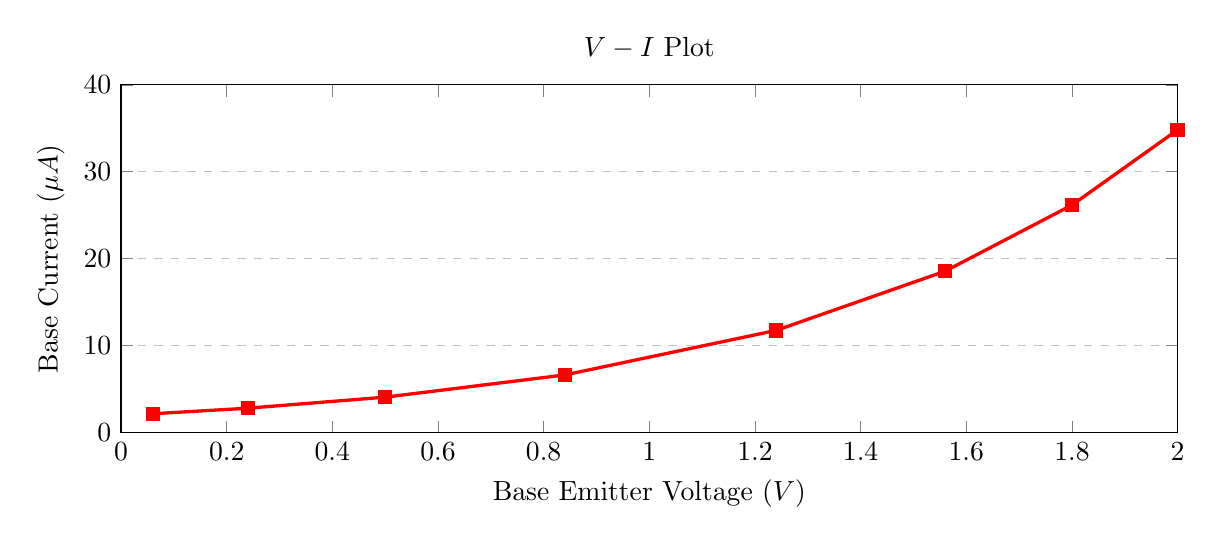
\begin{tikzpicture}
					\begin{axis}[
						title={$V - I$ Plot},
						width=15cm, height = 6cm,
						xlabel={Base Emitter Voltage ($V$)},
						ylabel={Base Current ($\mu A$)},
						xmin=0, xmax=2,
						ymin=0, ymax=40,
						xtick={0,0.2,0.4,0.6,0.8,1,1.2,1.4,1.6,1.8,2},
						ytick={0,10,20,30,40},
						legend pos=north west,
						ymajorgrids=true,
						grid style=dashed,
						%						legend entries = {Forward Biased Silicon Diode}
						]
						
						\addplot[
						color=red,very thick,mark = square*
						]
						coordinates {
							(0.06000, 2.179)
							(0.2400, 2.818)
							(0.5000, 4.085)
							(0.8400, 6.640)
							(1.240, 11.76)
							(1.560, 18.57)
							(1.800, 26.17)
							(2.000, 34.82)
						};					
					\end{axis}
				\end{tikzpicture}
				\caption{$V - I$ Plot of BJT Common Emitter - Input Characteristics at $V_{CE} = 1 V$}
			\end{figure}
		
		\newpage
		\subsection{BJT Common Emitter - Output Characteristics}
			\begin{figure}[h]
				\begin{longtable}[]{@{}lll@{}}
					\toprule
					Sr No. & Collector Voltage ($V$) & Collector Current ($mA$)\tabularnewline
					\midrule
					\endhead
					1 & 0.1000 & 7.427\tabularnewline
					2 & 1.500 & 67.45\tabularnewline
					3 & 2.800 & 73.97\tabularnewline
					4 & 3.900 & 74.46\tabularnewline
					5 & 5.000 & 74.51\tabularnewline
					6 & 6.000 & 74.52\tabularnewline
					7 & 7.800 & 74.52\tabularnewline
					8 & 9.000 & 74.52\tabularnewline
					9 & 10.00 & 74.52\tabularnewline
					\bottomrule
				\end{longtable}
				\caption{BJT Common Emmiter - Output Characteristics Table at $I_B = 15 \mu A$}
			\end{figure}
			
			\begin{figure}[h]
				\centering
				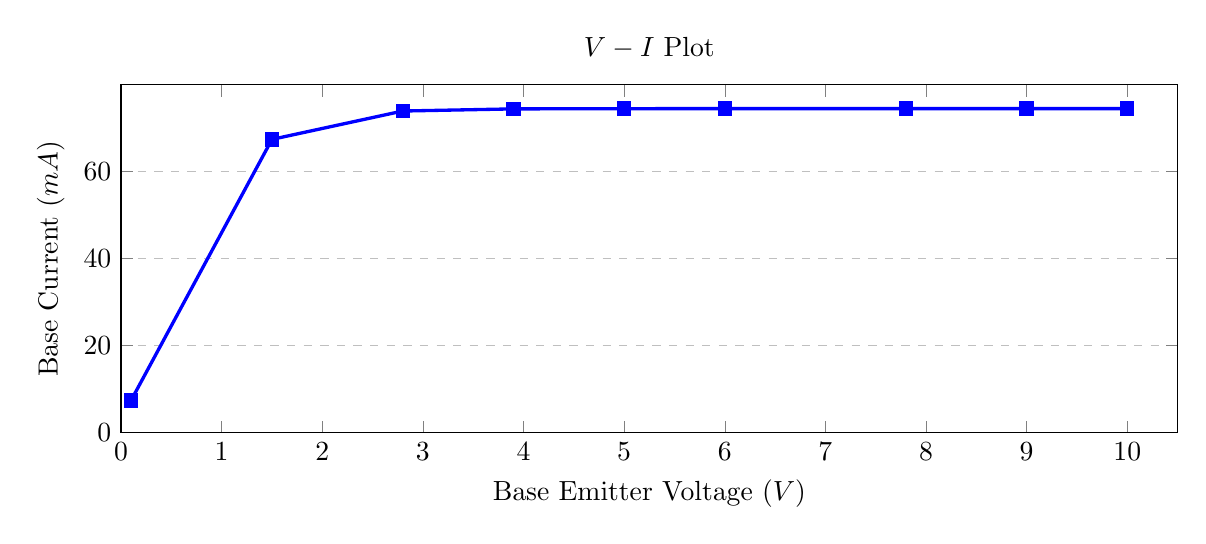
\begin{tikzpicture}
					\begin{axis}[
						title={$V - I$ Plot},
						width=15cm, height = 6cm,
						xlabel={Base Emitter Voltage ($V$)},
						ylabel={Base Current ($mA$)},
						xmin=0, xmax=10.5,
						ymin=0, ymax=80,
						xtick={0,1,2,3,4,5,6,7,8,9,10},
						ytick={0,20,40,60},
						legend pos=north west,
						ymajorgrids=true,
						grid style=dashed,
						%						legend entries = {Forward Biased Silicon Diode}
						]
						
						\addplot[
						color=blue,very thick,mark = square*
						]
						coordinates {
							(0.100, 7.427)
							(1.500, 67.45)
							(2.800, 73.97)
							(3.900, 74.46)
							(5.000, 74.51)
							(6.000, 74.52)
							(7.800, 74.52)
							(9.000, 74.52)
							(10.00, 74.52)
						};					
					\end{axis}
				\end{tikzpicture}
				\caption{$V - I$ Plot of BJT Common Emitter - Output Characteristics at $I_B = 15 \mu A$}
			\end{figure}
		
	\section{Result}
		A bipolar transistor allows a small current injected at one of its terminals to control a much larger current flowing between two other terminals, making the device capable of amplification or switching.The collector–emitter current can be viewed as being controlled by the base–emitter current (current control), or by the base–emitter voltage (voltage control). These views are related by the current–voltage relation of the base–emitter junction, which is the usual exponential current–voltage curve of a p–n junction (diode).